\documentclass[11pt,oneside]{article}

\usepackage[T1]{fontenc}
\usepackage[utf8]{inputenc}
\usepackage{amsmath,amsthm,mathtools}
\usepackage{newtxtext,newtxmath}
\usepackage{microtype}
\usepackage[a4paper,margin=27mm,headheight=15pt]{geometry}
\usepackage{booktabs,longtable,tabularx,array,multirow}
\usepackage{enumitem}
\usepackage{xcolor}
\usepackage[most]{tcolorbox}
\usepackage{tikz}
\usepackage{pgfplots}
\pgfplotsset{compat=1.18}
\usepackage{listings}
\usepackage{fancyhdr}
\usepackage{hyperref}
\usepackage[nameinlink,capitalise,noabbrev]{cleveref}
\usepackage{bookmark}

\definecolor{deepblue}{HTML}{174A7E}
\definecolor{deepgreen}{HTML}{276749}
\definecolor{deepred}{HTML}{9B2C2C}
\definecolor{warmgray}{HTML}{5B6573}
\definecolor{paleblue}{HTML}{EDF4FB}
\definecolor{palegreen}{HTML}{EDF8F2}
\definecolor{paleorange}{HTML}{FFF7E6}
\definecolor{palered}{HTML}{FFF1F0}

\hypersetup{
  colorlinks=true,
  linkcolor=deepblue,
  citecolor=deepgreen,
  urlcolor=deepblue,
  pdftitle={Critical-window and terminal-prime contraction for the Alaoglu--Erdos conjecture},
  pdfauthor={OpenAI GPT-5.6 Pro},
  pdfsubject={New progress on factorial cocycles associated with the Alaoglu--Erdos conjecture}
}

\pagestyle{fancy}
\fancyhf{}
\fancyhead[L]{Alaoglu--Erd\H{o}s: new progress report}
\fancyhead[R]{23 August 2026}
\fancyfoot[C]{\thepage}

\setlength{\parindent}{0pt}
\setlength{\parskip}{0.55em}
\setlist{itemsep=0.25em,topsep=0.35em}
\allowdisplaybreaks

\newtheorem{theorem}{Theorem}[section]
\newtheorem{proposition}[theorem]{Proposition}
\newtheorem{lemma}[theorem]{Lemma}
\newtheorem{corollary}[theorem]{Corollary}
\newtheorem{conjecture}[theorem]{Conjecture}
\newtheorem{problem}[theorem]{Problem}
\theoremstyle{definition}
\newtheorem{definition}[theorem]{Definition}
\newtheorem{example}[theorem]{Example}
\theoremstyle{remark}
\newtheorem{remark}[theorem]{Remark}

\newtcolorbox{newresult}[1][]{
  enhanced,breakable,colback=palegreen,colframe=deepgreen,
  boxrule=0.7pt,arc=1.5mm,left=2mm,right=2mm,top=1.5mm,bottom=1.5mm,
  title={New result#1},fonttitle=\bfseries
}
\newtcolorbox{imported}[1][]{
  enhanced,breakable,colback=paleblue,colframe=deepblue,
  boxrule=0.6pt,arc=1.5mm,left=2mm,right=2mm,top=1.5mm,bottom=1.5mm,
  title={Imported prerequisite#1},fonttitle=\bfseries
}
\newtcolorbox{opentarget}[1][]{
  enhanced,breakable,colback=paleorange,colframe=orange!70!black,
  boxrule=0.7pt,arc=1.5mm,left=2mm,right=2mm,top=1.5mm,bottom=1.5mm,
  title={Remaining target#1},fonttitle=\bfseries
}
\newtcolorbox{warningbox}[1][]{
  enhanced,breakable,colback=palered,colframe=deepred,
  boxrule=0.7pt,arc=1.5mm,left=2mm,right=2mm,top=1.5mm,bottom=1.5mm,
  title={Caution#1},fonttitle=\bfseries
}

\newcommand{\Z}{\mathbb Z}
\newcommand{\N}{\mathbb N}
\newcommand{\Q}{\mathbb Q}
\newcommand{\R}{\mathbb R}
\newcommand{\vp}[2]{v_{#1}\!\left(#2\right)}
\newcommand{\den}{\operatorname{den}}
\newcommand{\ord}{\operatorname{ord}}
\newcommand{\supp}{\operatorname{supp}}
\newcommand{\lc}{\operatorname{lc}}
\newcommand{\pos}[1]{#1^{+}}
\newcommand{\negp}[1]{#1^{-}}
\newcommand{\cstar}{c_{\!*}}
\newcommand{\thetas}{\vartheta}
\newcommand{\FF}{\mathcal F}
\newcommand{\BB}{\mathcal B}
\newcommand{\TT}{\mathcal T}
\newcommand{\bigO}{\mathcal O}

\lstset{
  basicstyle=\ttfamily\small,
  columns=fullflexible,
  frame=single,
  breaklines=true,
  showstringspaces=false,
  keywordstyle=\bfseries,
  commentstyle=\itshape\color{warmgray}
}

\title{\textbf{Critical-Window and Terminal-Prime Contraction\\
for the Alaoglu--Erd\H{o}s Conjecture}\\[0.5em]
\large A nonduplicative progress report beyond the unified report}
\author{OpenAI GPT-5.6 Pro}
\date{23 August 2026}

\begin{document}
\maketitle

\begin{abstract}
Assume hypothetically that $x\in\R\setminus\Z$ and
$M=2^x$, $A=3^x$ are integers.  The attached unified report introduced the
falling-factorial cocycles
\[
 F_n=(A^n)_{M^n}=\frac{A^n!}{(A^n-M^n)!},
 \qquad
 \FF_{P,n}=\prod_j F_{n+j}^{c_j},
 \quad P(T)=\sum_jc_jT^j,
\]
and reduced their archimedean near-unit property to the annihilations
$P(M)=P'(M)=P(M^2/A)=0$.  It left a linear-width feasibility problem:
could a varying annihilator $P=P_n$ make $\FF_{P,n}$ both integral and
asymptotic to $1$ after crossing the prime-window span threshold?

This report closes that feasibility problem negatively.  The key is not a sharper estimate
for one highest negative coefficient, but a simultaneous sum over the terminal-prime window
attached to \emph{every} negative coefficient.  Integrality forces each negative
$M$-weighted coefficient mass to be transported upward.  The transport operator has norm at
most
\[
 \kappa_n=
 \frac{2(M/A)^n}{1-M/A}+\frac{2}{M-1}
 +\frac{2M}{n(M-1)^2}=o(1)+\frac{2}{M-1},
\]
whereas $P(M)=0$ says that the total positive and negative $M$-weighted masses are exactly
equal.  Since the independently verified finite region gives $M\ge2^{14}$, one has
$\kappa_n<1$; hence no nonzero integer polynomial with $P(M)=0$ can produce an integral
falling-factorial cocycle for all sufficiently large $n$.  The argument is uniform in the
degree, span, coefficient height, and number of sign changes.  It also applies to binomial
cocycles.

Two supporting results are developed.  First, the earlier prime-window theorem is sharpened
from a fixed linear margin to any additive margin tending to infinity.  Second, confluent
Hermite interpolation identifies the canonical maximal-contact stencils and proves an exact
``terminal-prime multiplicity mismatch'': a double root at $M$ forces a boundary coefficient
at least $(D+1)M^D$, while a transported terminal interval supplies only
$O((M/A)^tM^D)$ copies of each terminal prime.  These results explain why the apparent
critical Hermite families cannot escape.  They do not prove the Alaoglu--Erd\H{o}s conjecture;
they remove one of the unified report's four explicit open directions and leave a more
focused search for a genuinely primitive-sensitive mechanism.
\end{abstract}

\begin{newresult}[ --- headline]
The main theorem, \Cref{thm:global-contraction}, gives a degree-free negative solution of the
unified report's ``linear-width factorial feasibility'' target.  It uses only the imported
candidate identities, Huxley's theorem on primes in short intervals, elementary valuation
bounds, and the exact mass balance $P(M)=0$.
\end{newresult}

\tableofcontents
\newpage

\section{Scope, audit boundary, and status}
\label{sec:scope}

This document is deliberately not another survey of the conjecture.  The attached unified
report is more than twenty-three thousand lines long and already treats the standard
transcendence, Kummer, determinant, interpolation, spectral, dynamical, $p$-adic, and
formalization routes.  Repeating those sections would conceal rather than clarify new
progress.  We import only the small interface needed below.

\begin{imported}
Under failure of the conjecture, choose the least nonintegral solution (or simply fix any
hypothetical nonintegral solution) and put
\[
 M=2^x\in\Z_{>0},\qquad A=3^x\in\Z_{>0}.
\]
Then
\[
 \frac{\log M}{\log A}=\frac{\log2}{\log3}=:\alpha,
 \qquad \frac12<\alpha<\frac23,
 \qquad 1<M<A.
\]
The kernel-checked finite region in the attached report gives $x\ge14$, hence
$M\ge2^{14}$ and
\[
 q:=\frac MA=\left(\frac23\right)^x
 \le\left(\frac23\right)^{14}=0.0034254873\ldots.
\]
The report also proved the fixed-polynomial near-unit classification for the factorial
cocycles used here.
\end{imported}

The following status terminology is used.

\begin{center}
\begin{tabularx}{0.94\textwidth}{>{\bfseries}lX}
\toprule
Imported & proved or kernel-checked in the attached unified report; not reproved in full.\\
New theorem & proved in this report at the paper level.\\
Known analytic input & a classical external theorem, principally Huxley's short-interval
prime theorem or Brun--Titchmarsh.\\
Open target & a precisely stated step not proved here.\\
\bottomrule
\end{tabularx}
\end{center}

The main new theorem is control-blind: it applies equally to the genuine integer-exponent
pairs $(2^m,3^m)$.  That is appropriate because it is a \emph{negative closure} of an
auxiliary strategy, not a proof of the conjecture.  A final proof must still use information
that distinguishes a primitive hypothetical pair from the controls, such as an external
support prime, least-generator structure, or the saturated rational-output spectrum.

\section{Factorial cocycles and the first decay modes}
\label{sec:factorial-setup}

Set
\[
 N_n=A^n,\qquad K_n=M^n,
 \qquad
 F_n=(N_n)_{K_n}=N_n(N_n-1)\cdots(N_n-K_n+1).
\]
For a nonzero polynomial $P(T)=\sum_{j=0}^dc_jT^j\in\Z[T]$ define
\[
 \FF_{P,n}=\prod_{j=0}^dF_{n+j}^{c_j}.
\]
The expression is a positive rational number, and
\[
 \vp p{\FF_{P,n}}=\sum_jc_jV_p(n+j),
 \qquad
 V_p(t):=\vp p{F_t}.
\]

The mode notation used below is
\[
 \lambda=\frac{M^2}{A}>1,
 \quad
 \eta=\frac{M^3}{A^2}<1,
 \quad
 q=\frac MA<1,
 \quad
 \tau=\frac{M^4}{A^3}<q,
 \quad
 \sigma=\left(\frac MA\right)^2<\tau,
 \quad
 \upsilon=\frac{M^5}{A^4}<\sigma.
\]
Their order follows from the elementary base inequalities
$4>3$, $8<9$, $2/3>16/27>4/9>32/81$.

\begin{lemma}[Six-term factorial expansion]
\label{lem:six-mode}
As $n\to\infty$,
\begin{align}
 \log F_n={}&nM^n\log A-\frac12\lambda^n-\frac16\eta^n
 +\frac12q^n-\frac1{12}\tau^n+\frac14\sigma^n
 +O(\upsilon^n).                                    \label{eq:six-mode}
\end{align}
The implied constant depends only on $M,A$.
\end{lemma}

\begin{proof}
Write $N=A^n$, $K=M^n$, and $u=K/N=q^n$.  Then
\[
 \log F_n=K\log N+\sum_{j=0}^{K-1}\log\left(1-\frac jN\right).
\]
For $0\le y\le u<1/2$,
\[
 \log(1-y)=-y-\frac{y^2}{2}-\frac{y^3}{3}
 +O\left(\frac{y^4}{1-u}\right).
\]
Using
\begin{align*}
 \sum_{j<K}j&=\frac{K^2-K}{2},\\
 \sum_{j<K}j^2&=\frac{2K^3-3K^2+K}{6},\\
 \sum_{j<K}j^3&=\frac{K^4-2K^3+K^2}{4},
\end{align*}
produces the displayed modes.  The Taylor remainder is
$O(K^5/N^4)=O(\upsilon^n)$.  The omitted lower-power terms from the three displayed power
sums have bases at most $(8/27)^x< (32/81)^x$, so they are absorbed by the same error.
\end{proof}

Let $E$ denote the forward shift.  The identities
\[
 P(E)(\rho^n)=P(\rho)\rho^n,
 \qquad
 P(E)(n\rho^n)=\rho^n\bigl(nP(\rho)+\rho P'(\rho)\bigr)
\]
show why the imported near-unit classification begins with
\[
 P(M)=P'(M)=P(\lambda)=0.                    \label{eq:basic-annihilation}
\]
For a fixed $P$, these conditions remove the visible term and the unique divergent collision
mode.  The remaining leading mode is usually $\eta^n$.  Varying $P=P_n$ can cancel further
modes, but its coefficients and degree then grow, and uniformity becomes the entire issue.

\section{Terminal-prime windows}
\label{sec:windows}

For an index $t$ put
\[
 X_t=A^t,\qquad H_t=M^t=X_t^\alpha,
 \qquad I_t=(X_t-H_t,X_t].
\]
Huxley's theorem applies because
\[
 \alpha=\frac{\log2}{\log3}=0.6309297535\ldots>\frac7{12}.
\]
Consequently
\begin{equation}
 \thetas(X_t)-\thetas(X_t-H_t)=(1+o(1))H_t,
 \label{eq:huxley-window}
\end{equation}
where $\thetas(y)=\sum_{p\le y}\log p$.  In particular, $I_t$ contains primes for every
sufficiently large $t$.

A prime in $I_t$ occurs in exactly one place in the base factorial $F_t$.  Its possible
reappearance in a higher factorial is controlled uniformly as follows.

\begin{lemma}[Transported terminal-prime valuation]
\label{lem:transport-bound}
There is $t_0=t_0(M,A)$ such that for every $t\ge t_0$, every prime $p\in I_t$, and every
integer $\ell\ge1$,
\begin{equation}
 V_p(t+\ell)
 \le 2q^tM^\ell+2\left(1+\frac\ell t\right).          \label{eq:transport-bound}
\end{equation}
Moreover $V_p(t)=1$, and $V_p(s)=0$ for $0\le s<t$.
\end{lemma}

\begin{proof}
For large $t$ one has $p>X_t-H_t>X_t/2$, so $p$ and no other multiple of $p$ lies in the
terminal interval defining $F_t$, and $p^2>X_t$.  Also
$A^{t-1}<A^t-M^t$, so no lower factorial contains $p$.

For $s=t+\ell$, put $Y=A^s$, $W=M^s$.  Legendre's interval formula gives
\[
 V_p(s)=\sum_{r\ge1}
 \left(\left\lfloor\frac{Y}{p^r}\right\rfloor
 -\left\lfloor\frac{Y-W}{p^r}\right\rfloor\right).
\]
Each nonzero summand is at most $W/p^r+1$.  Hence
\[
 V_p(s)\le\frac{W}{p-1}+\frac{\log Y}{\log p}.
\]
Since $p\ge A^t(1-q^t)$, the first term is at most $2q^tM^\ell$ for large $t$.  The second is
at most $2(1+\ell/t)$, again uniformly for large $t$.
\end{proof}

The first term in \eqref{eq:transport-bound} is the expected number of transported multiples.
The second is the crude one-per-prime-power allowance.  After $M$-weighting and summing over
coefficient indices, both kernels are summable.  This observation is the decisive step.

\section{The global terminal-prime contraction}
\label{sec:contraction}

For a coefficient $c_j$ write $c_j^+=\max(c_j,0)$ and
$c_j^-=\max(-c_j,0)$.  Define the positive and negative $M$-weighted masses
\[
 S_+(P)=\sum_jc_j^+M^j,
 \qquad
 S_-(P)=\sum_jc_j^-M^j.
\]
If $P(M)=0$, then
\begin{equation}
 S_+(P)=S_-(P)>0.                              \label{eq:mass-balance}
\end{equation}
The strict positivity follows because a nonzero polynomial with positive argument $M$ cannot
vanish when all its coefficients have the same sign.

\begin{theorem}[Global terminal-prime contraction]
\label{thm:global-contraction}
Let $M,A$ arise from a hypothetical nonintegral solution, so in particular $M\ge2^{14}$ and
$q=M/A$.  There exists $n_0=n_0(M,A)$ such that the following holds for every $n\ge n_0$.
If $P\in\Z[T]\setminus\{0\}$ satisfies $P(M)=0$, then
\[
 \FF_{P,n}\notin\Z.
\]
The conclusion is uniform in the degree, span, coefficient height, and sign pattern of $P$.
More precisely, for some negative coefficient index $k$ every prime in $I_{n+k}$ occurs in
the reduced denominator of $\FF_{P,n}$, and therefore
\begin{equation}
 \log\den(\FF_{P,n})\ge(1-o(1))M^{n+k}\ge(1-o(1))M^n. \label{eq:global-den-lower}
\end{equation}
The $o(1)$ is along $n+k\to\infty$.
\end{theorem}

\begin{proof}
Assume for contradiction that $\FF_{P,n}$ is an integer.  Fix an index $k$ with $c_k<0$ and
choose a prime $p\in I_{n+k}$, which exists for all sufficiently large $n$ by
\eqref{eq:huxley-window}.  Put $t=n+k$.  By \Cref{lem:transport-bound}, $p$ occurs once in
$F_t$, occurs in no lower factor, and satisfies the displayed upper bound in every higher
factor.  Higher negative coefficients only make the valuation smaller, so integrality implies
\begin{align}
 c_k^- &\le
 \sum_{j>k}c_j^+V_p(n+j)                                                   \notag\\
 &\le 2q^{n+k}\sum_{j>k}c_j^+M^{j-k}
 +2\sum_{j>k}c_j^+\left(1+\frac{j-k}{n+k}\right).          \label{eq:one-negative-transport}
\end{align}
Multiply by $M^k$ and sum \eqref{eq:one-negative-transport} over all negative indices $k$.
For the transported-multiple term, if
$T_k=\sum_{j>k}c_j^+M^j\le S_+(P)$, then
\begin{align}
 2\sum_{c_k<0}q^{n+k}T_k
 &\le2q^nS_+(P)\sum_{k\ge0}q^k
 =\frac{2q^n}{1-q}S_+(P).                         \label{eq:first-contraction}
\end{align}
For the prime-power allowance, interchange the order of summation.  Since $n+k\ge n$,
\begin{align}
 &2\sum_{c_k<0}\sum_{j>k}c_j^+M^k
 \left(1+\frac{j-k}{n+k}\right)                                      \notag\\
 &\quad\le2\sum_{c_j>0}c_jM^j
 \sum_{\ell\ge1}M^{-\ell}\left(1+\frac\ell n\right)                  \notag\\
 &\quad=2S_+(P)\left(\frac1{M-1}+\frac{M}{n(M-1)^2}\right).             \label{eq:second-contraction}
\end{align}
Combining \eqref{eq:mass-balance}--\eqref{eq:second-contraction} gives
\begin{equation}
 1\le\kappa_n:=
 \frac{2q^n}{1-q}+\frac{2}{M-1}+\frac{2M}{n(M-1)^2}.                    \label{eq:kappa}
\end{equation}
But $M\ge2^{14}$ and $q\le(2/3)^{14}$, so $\kappa_n<1$ (indeed
$\kappa_1<0.0072$ at the extremal values, and it decreases with $n$).  This contradiction proves nonintegrality.

For the quantitative statement, observe that if the right-hand side of
\eqref{eq:one-negative-transport} dominated $c_k^-$ for every negative $k$, the preceding
summation would again give \eqref{eq:kappa}.  Hence for some $k$ the strict reverse inequality
holds.  The bound in \Cref{lem:transport-bound} is uniform over $p\in I_{n+k}$, so every such
prime has negative valuation in $\FF_{P,n}$.  Summing their logarithms and applying
\eqref{eq:huxley-window} gives \eqref{eq:global-den-lower}.
\end{proof}

\begin{newresult}[ --- closure of the factorial target]
The theorem needs only $P(M)=0$, one of the three archimedean annihilations.  It therefore
rules out, for all sufficiently large $n$, every polynomial contemplated by the unified
report's linear-width factorial feasibility target.  No choice of degree, critical span,
coefficient height, additional mode cancellations, or structural-prime congruences can make
that particular falling-factorial cocycle integral.
\end{newresult}

Several features deserve emphasis.

\begin{enumerate}[label=(\roman*)]
\item The proof does not pick the highest negative coefficient.  It uses the terminal window
for every negative coefficient and then invokes the exact global balance $P(M)=0$.
\item There is no factor equal to the number of negative coefficients: the geometric weights
$q^k$ sum to $(1-q)^{-1}$.  This is why the theorem remains uniform even when the degree is
very large.
\item The additive ``one per prime power'' error is not accumulated as a degree factor either;
after $M$-weighting its kernel is $M^{-\ell}$, whose first two moments are explicit.
\item The finite exclusion $M\ge2^{14}$ is far more than is needed.  Asymptotically the
contraction requires essentially $2/(M-1)<1$, together with sufficiently small $q^n$.
\end{enumerate}

\begin{corollary}[No integral near-unit factorial cocycles]
\label{cor:no-factorial-near-unit}
There is no sequence $P_n\in\Z[T]\setminus\{0\}$ such that, for all sufficiently large $n$,
\[
 P_n(M)=P_n'(M)=P_n(M^2/A)=0,
 \qquad \FF_{P_n,n}\in\Z,
 \qquad \FF_{P_n,n}\longrightarrow1.
\]
The conclusion remains true after imposing any additional exact mode cancellations.
\end{corollary}

\begin{proof}
The first displayed equality is already enough for \Cref{thm:global-contraction}.
\end{proof}

\subsection{Binomial and occupancy-normalized variants}

Put
\[
 B_n=\binom{A^n}{M^n}=\frac{F_n}{M^n!},
 \qquad
 R_n=\frac{F_n}{(A^n)^{M^n}}.
\]
For $p\in I_t$ one has $p>M^t$, hence $\vp p{M^t!}=0$ and
$\vp p{B_t}=\vp p{R_t}=1$.  At a higher index,
\[
 \vp p{B_s}\le V_p(s),\qquad \vp p{R_s}=V_p(s),
\]
because the normalizing factors introduce no new positive high-prime valuation.  The same
contraction proof therefore gives the following.

\begin{corollary}[Binomial and no-collision closure]
\label{cor:binomial-closure}
For all sufficiently large $n$ and every nonzero $P\in\Z[T]$ with $P(M)=0$, neither
\[
 \prod_jB_{n+j}^{c_j}
 \quad\text{nor}\quad
 \prod_jR_{n+j}^{c_j}
\]
is an integer.  In particular, the binomial-cocycle variant of the linear-width target is
also infeasible.
\end{corollary}

\section{A critical-window sharpening}
\label{sec:critical-window}

The global contraction supersedes the span analysis for the factorial target.  Nevertheless,
a sharper form of the earlier prime-window theorem is independently useful: the fixed
linear margin $\varepsilon n$ can be replaced by any additive margin tending to infinity.
This identifies the genuinely critical boundary before the global mass balance is used.

Let $k_n$ be the highest negative coefficient index of $P_n$, let $d_n=\deg P_n$, and put
\[
 t_n=n+k_n,
 \qquad D_n=d_n-k_n,
 \qquad
 \cstar=\log_2\frac32=\log_23-1=0.5849625007\ldots.
\]
Also set
\[
 \delta_0=2-\log_23=0.4150374993\ldots,
 \qquad
 \Delta_0=1-\frac{8q}{\delta_0(1-q)}.
\]
For $x\ge14$, $\Delta_0\ge0.9337$.

\begin{theorem}[Additive critical-window obstruction]
\label{thm:additive-window}
Let $P_n\in\Z[T]$ be nonzero and have a negative coefficient.  Suppose $t_n\to\infty$ and
there is a sequence $h_n\to\infty$ such that
\begin{equation}
 D_n\le\cstar t_n-h_n.                              \label{eq:additive-window-hyp}
\end{equation}
Then
\begin{equation}
 \log\den(\FF_{P_n,n})
 \ge(-c_{n,k_n})(\Delta_0-o(1))M^{t_n}.              \label{eq:additive-window-concl}
\end{equation}
In particular, an integral factorial cocycle must satisfy
$D_n\ge\cstar t_n-O(1)$.
\end{theorem}

\begin{proof}
The proof follows the prime-window argument imported from the unified report; only the
boundary bookkeeping changes.  Put $X=A^{t_n}$ and $H=M^{t_n}$.  A prime in $(X-H,X]$ is
lost from the denominator only if some higher positive factor captures a transported
multiple.  At relative shift $\ell$, the relevant prime interval has length
$O(Hq^\ell)$, and the number of possible multipliers is
$O(1+A^\ell H/X)$.

The minimum logarithmic thickness occurs at $\ell=D_n$.  Using
$\cstar=-\log q/\log M$ and \eqref{eq:additive-window-hyp},
\begin{align*}
 \frac{\log(Hq^{D_n})}{\log X}
 &\ge \frac{t_n\log M+(\cstar t_n-h_n)\log q}{t_n\log A}\\
 &=\delta_0+\frac{h_n(\log A-\log M)}{t_n\log A}
 \ge\delta_0.
\end{align*}
Thus Brun--Titchmarsh may be applied with any fixed $\delta<\delta_0$ for all large $n$.
The first multiplier sum covers at most
\[
 \left(\frac{8q}{\delta(1-q)}+o(1)\right)H
\]
of logarithmic prime mass.  The drifting-multiplier sum is smaller by the factor
\[
 q^{t_n}M^{D_n}\le M^{-h_n}\longrightarrow0,
\]
which is exactly where a divergent additive margin replaces the earlier fixed
$\varepsilon t_n$.  Huxley's theorem supplies total mass $(1+o(1))H$.  Letting
$\delta\uparrow\delta_0$ proves \eqref{eq:additive-window-concl}.
\end{proof}

\begin{remark}
The theorem leaves only a bounded additive strip
$D_n=\cstar t_n+O(1)$.  Canonical Hermite stencils initially appear capable of living in this
strip.  The next sections show why coefficient multiplicity, and ultimately the global
contraction, destroys that appearance.
\end{remark}

\section{Coefficient-sensitive prime-window duality}
\label{sec:coefficient-dual}

The span theorem records whether a higher factor can capture a terminal prime at least once.
It ignores how many copies are needed.  If the negative coefficient is much larger than the
positive coefficient attached to the transported interval, a captured prime can still remain
in the denominator.  \Cref{lem:transport-bound} yields an explicit coefficient-sensitive
dual certificate.

For a polynomial $P=\sum c_jT^j$ and a negative index $k$, define
\begin{equation}
 \Psi_{n,k}(P):=c_k^--
 \sum_{j>k}c_j^+
 \left[2q^{n+k}M^{j-k}+2\left(1+\frac{j-k}{n+k}\right)\right].           \label{eq:Psi}
\end{equation}

\begin{proposition}[Window-dominance certificate]
\label{prop:window-dominance}
If $\Psi_{n,k}(P)>0$ and $n+k$ is sufficiently large, then every prime in $I_{n+k}$ has
negative valuation in $\FF_{P,n}$.  Consequently
\[
 \log\den(\FF_{P,n})\ge(1-o(1))M^{n+k}.
\]
\end{proposition}

\begin{proof}
For $p\in I_{n+k}$, lower factors are absent, the factor at $k$ contributes $-c_k^-$, higher
negative coefficients may be discarded in an upper bound, and higher positive coefficients
are bounded by \Cref{lem:transport-bound}.  Thus
$\vp p{\FF_{P,n}}\le-\Psi_{n,k}(P)<0$.  Sum $\log p$ and use Huxley.
\end{proof}

The proof of \Cref{thm:global-contraction} can now be read as a Farkas-type statement: if all
window-dominance certificates failed, their $M^k$-weighted sum would imply
$S_-(P)\le\kappa_nS_+(P)$, contradicting $P(M)=0$.  Hence at least one of the explicit rows
\eqref{eq:Psi} separates the coefficient vector from the valuation cone.

\begin{corollary}[Necessary tail inflation without mass balance]
\label{cor:tail-inflation}
If $\FF_{P,n}$ is an integer and $c_k<0$, then
\[
 c_k^-\le
 2q^{n+k}\sum_{j>k}c_j^+M^{j-k}
 +2\sum_{j>k}c_j^+\left(1+\frac{j-k}{n+k}\right).
\]
Unless the prime-power allowance dominates, the $M$-weighted positive tail above $k$ must
exceed $c_k^-$ by a factor of order $q^{-(n+k)}$.
\end{corollary}

This coefficient inflation is the feature missed by a support-only prime-window count.  It is
also the right diagnostic for exact LP computations: a candidate ray should be rejected
before any prime enumeration if one of the inexpensive inequalities \eqref{eq:Psi} is
positive.

\section{Confluent Hermite tails and complete homogeneous functions}
\label{sec:hermite}

The canonical way to cancel a prescribed finite list of factorial modes while keeping a
single high-degree monomial is Hermite interpolation.  This section makes that construction
exact and shows how the terminal-prime certificate sees it.

Let $\mathcal R=(r_1,\ldots,r_d)$ be a multiset of positive rational numbers, with repeated
entries interpreted confluently.  In the applications it contains $M$ twice and begins with
\[
 (M,M,\lambda),\quad
 (M,M,\lambda,\eta),\quad
 (M,M,\lambda,\eta,q),\quad\ldots.
\]
For a polynomial $G$, let $H_{\mathcal R}G$ be the unique polynomial of degree $<d$ that
matches $G$ and the required derivatives at the repeated nodes.  Thus
$G-H_{\mathcal R}G$ is divisible over $\Q[T]$ by
\[
 D_{\mathcal R}(T)=\prod_{i=1}^d(T-r_i).
\]

Let $h_m(y_1,\ldots,y_s)$ denote the complete homogeneous symmetric polynomial of degree
$m$, with $h_0=1$.

\begin{lemma}[Hermite boundary coefficient]
\label{lem:hermite-boundary}
For $e\ge d-1$, the coefficient of $T^{d-1}$ in $H_{\mathcal R}(T^e)$ is
\[
 [r_1,\ldots,r_d]T^e=h_{e-d+1}(r_1,\ldots,r_d).
\]
If $\mathcal R$ contains $M$ twice, then for every $\ell\ge0$,
\begin{equation}
 h_\ell(\mathcal R)\ge(\ell+1)M^\ell.                \label{eq:h-lower}
\end{equation}
\end{lemma}

\begin{proof}
The divided-difference identity follows, for example, by comparing coefficients in
\[
 \prod_{i=1}^d\frac1{1-r_i z}=\sum_{m\ge0}h_m(r_1,\ldots,r_d)z^m
\]
or by induction in the Newton interpolation formula; confluence follows by continuity.
For \eqref{eq:h-lower}, retain only the $\ell+1$ monomials obtained by distributing total
degree $\ell$ between the two copies of $M$ and assigning degree zero to all other variables.
\end{proof}

A related exact evaluation formula is useful.

\begin{proposition}[Hermite remainder identity]
\label{prop:hermite-remainder}
For $N\ge d$ let
\[
 P_{\mathcal R,N}(T)=T^N-H_{\mathcal R}(T^N).
\]
Then, for every $z$,
\begin{equation}
 P_{\mathcal R,N}(z)=D_{\mathcal R}(z)
 h_{N-d}(z,r_1,\ldots,r_d).                           \label{eq:hermite-remainder}
\end{equation}
Moreover the coefficient of $T^{d-1}$ is
$-h_{N-d+1}(\mathcal R)$.
\end{proposition}

\begin{proof}
Polynomial division of $T^N$ by the monic polynomial $D_{\mathcal R}$ gives a quotient whose
generating function is the complete homogeneous series.  Equivalently, both sides of
\eqref{eq:hermite-remainder} are monic degree-$N$ polynomials with the same confluent zeros
and the same quotient recurrence.  The boundary coefficient is
\Cref{lem:hermite-boundary}.
\end{proof}

Because $P_{\mathcal R,N}$ has $d$ positive roots counted with multiplicity and at most
$d+1$ nonzero coefficients (the degrees $0,\ldots,d-1,N$), Descartes' rule forces every low
coefficient to be nonzero and the signs to alternate.  In particular the highest low
coefficient, at degree $d-1$, is negative.

The construction extends from one high monomial to an arbitrary nonnegative high tail.

\begin{definition}[Positive-tail Hermite annihilator]
Let
\[
 G(T)=\sum_{e\ge d}a_eT^e,
 \qquad a_e\in\Q_{\ge0},
 \qquad G\ne0,
\]
with finite support, and put
\[
 P(T)=G(T)-H_{\mathcal R}G(T).
\]
After multiplying by a positive integer, suppose $P\in\Z[T]$.  Then $P$ is called a
positive-tail Hermite annihilator for $\mathcal R$.
\end{definition}

Its coefficient at $T^{d-1}$ is exactly
\begin{equation}
 c_{d-1}=-\sum_{e\ge d}a_eh_{e-d+1}(\mathcal R),       \label{eq:positive-tail-boundary}
\end{equation}
whereas all coefficients above degree $d-1$ are the nonnegative $a_e$.

\section{Terminal-prime multiplicity mismatch for Hermite tails}
\label{sec:hermite-nogo}

The next theorem is subsumed by the global contraction, but it exposes the exact local
mechanism and remains useful for symbolic dual certificates.

\begin{theorem}[Positive-tail Hermite no-go]
\label{thm:hermite-nogo}
Let $\mathcal R$ be any finite multiset of positive rational nodes containing $M$ twice, and
let $P\in\Z[T]$ be a nonzero positive-tail Hermite annihilator for $\mathcal R$.  Then for all
sufficiently large $n$, $\FF_{P,n}$ is not an integer.  More precisely, every prime in
$I_{n+d-1}$ occurs in its denominator.
\end{theorem}

\begin{proof}
Put $t=n+d-1$ and write $\ell=e-d+1\ge1$.  By
\eqref{eq:positive-tail-boundary} and \eqref{eq:h-lower}, the negative boundary coefficient
has magnitude at least
\[
 c_{d-1}^-\ge\sum_{e\ge d}a_e(\ell+1)M^\ell.
\]
For a prime $p\in I_t$, the only positive contributions come from the high tail, and
\Cref{lem:transport-bound} bounds them by
\[
 \sum_{e\ge d}a_e
 \left[2q^tM^\ell+2\left(1+\frac\ell t\right)\right].
\]
Since $M\ge2^{14}$ and $q^t\to0$, for every $\ell\ge1$ and all large $t$ one has
\[
 (\ell+1)M^\ell>
 2q^tM^\ell+2\left(1+\frac\ell t\right).
\]
Thus the boundary negative multiplicity cannot be supplied by the transported positive tail,
and the valuation is negative for every $p\in I_t$.
\end{proof}

For the one-spike stencil $P_{\mathcal R,N}$, put $D=N-d+1$.  The ratio of the negative
boundary coefficient to the top coefficient is
\[
 h_D(\mathcal R)\ge(D+1)M^D,
\]
while the top factorial contains at most
$O(q^tM^D+1+D/t)$ copies of a terminal prime.  The common factor $M^D$ cancels in the
comparison; the remaining ratio is essentially $(D+1)/q^t$, so increasing the span only
makes the multiplicity mismatch worse.

\begin{corollary}[All isolated-top maximal-contact families are closed]
\label{cor:all-hermite-closed}
Choose any finite or varying list of additional positive factorial modes, append it to the
confluent root list $(M,M,\lambda)$, and form the primitive integer multiple of
$T^N-H_{\mathcal R}(T^N)$.  Its factorial cocycle is nonintegral for all sufficiently large
$n$, regardless of how $N$, the number of cancelled modes, or the coefficients vary.
\end{corollary}

This includes the initially promising families that cancel $\eta$, then $q$, then $\tau$,
and so on.  The obstruction is stronger than rational-root denominator growth and stronger
than the critical-span theorem: it does not require archimedean near-unit estimates at all.

\section{The apparent mode phase diagram}
\label{sec:phase-diagram}

It is still instructive to record why the Hermite route looked promising before the
multiplicity mismatch was included.  Put
\[
 R=\frac{\log A}{\log M}=\log_23=1.5849625007\ldots,
 \qquad \cstar=R-1.
\]
For a subunit mode $\rho=M^s/A^r$, define its normalized decay deficit
\[
 \delta(\rho)=\log_M(1/\rho)=rR-s>0.
\]
The first modes from \Cref{lem:six-mode} have the following data.

\begin{center}
\begin{tabular}{ccllll}
\toprule
rank & mode & $(r,s)$ & coefficient & $\delta$ & numerical value\\
\midrule
1 & $\eta=M^3/A^2$ & $(2,3)$ & $-1/6$ & $2R-3$ & $0.1699250$\\
2 & $q=M/A$ & $(1,1)$ & $+1/2$ & $R-1$ & $0.5849625$\\
3 & $\tau=M^4/A^3$ & $(3,4)$ & $-1/12$ & $3R-4$ & $0.7548875$\\
4 & $\sigma=M^2/A^2$ & $(2,2)$ & $+1/4$ & $2R-2$ & $1.1699250$\\
5 & $\upsilon=M^5/A^4$ & $(4,5)$ & $-1/20$ & $4R-5$ & $1.3398500$\\
\bottomrule
\end{tabular}
\end{center}

Suppose a one-spike Hermite stencil cancels all modes through a subunit root $\rho$.  If
$\rho=u/v$ in lowest terms and the low footprint has fixed degree, evaluating the integer
stencil at $u/v$ gives the elementary gap divisibility
\[
 v^D\mid \lc(P),
\]
where $D$ is the exponent gap between the isolated top monomial and the low footprint.  Since
$v\ge1/\rho$, the primitive leading coefficient costs at least $\rho^{-D}$.  If $\rho_-$ is
the last cancelled mode and $\rho_+$ the first uncancelled mode, the naively available slope
is therefore at most
\begin{equation}
 \frac{\delta(\rho_+)}{1+\delta(\rho_-)}.              \label{eq:naive-slope}
\end{equation}
The first values are
\begin{center}
\begin{tabular}{llll}
\toprule
last cancelled & first surviving & bound from \eqref{eq:naive-slope} & comparison with $\cstar$\\
\midrule
none & $\eta$ & $0.1699250$ & below\\
$\eta$ & $q$ & $1/2$ & below\\
$q$ & $\tau$ & $0.4762810$ & below\\
$\tau$ & $\sigma$ & $2/3$ & \emph{above}\\
$\sigma$ & $\upsilon$ & $0.6174638$ & \emph{above}\\
\bottomrule
\end{tabular}
\end{center}

Thus the first scalar-height calculation not automatically killed by the prime threshold is
the stencil cancelling $\eta,q,\tau$, whose first surviving mode is $\sigma$.  This is the
``first surviving seven-term stencil'' found during the present investigation.  It does not
actually survive: \Cref{thm:hermite-nogo} shows that its highest low negative coefficient
requires $(D+1)M^D$ copies of each terminal prime, while all transported positive factors
supply only $O(q^tM^D)$.  The global contraction then closes every non-Hermite variation as
well, provided $P(M)=0$ and integrality is demanded.

\begin{figure}[ht]
\centering
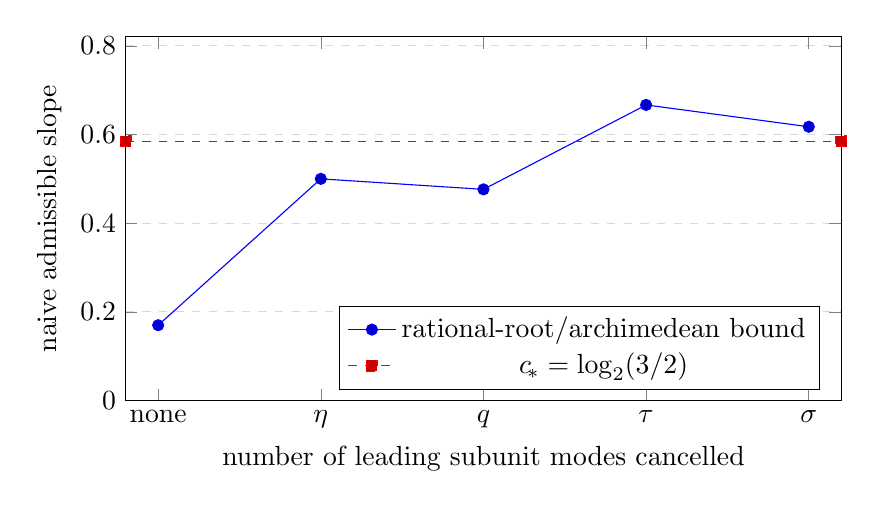
\begin{tikzpicture}
\begin{axis}[
  width=0.88\textwidth,height=6.2cm,
  xlabel={number of leading subunit modes cancelled},
  ylabel={naive admissible slope},
  xmin=-0.2,xmax=4.2,ymin=0,ymax=0.82,
  xtick={0,1,2,3,4},
  xticklabels={none,$\eta$,$q$,$\tau$,$\sigma$},
  ymajorgrids=true,grid style={dashed,gray!30},
  legend pos=south east]
\addplot+[mark=*] coordinates {
 (0,0.1699250014)
 (1,0.5)
 (2,0.4762809857)
 (3,0.6666666667)
 (4,0.6174637806)
};
\addplot+[domain=-0.2:4.2,samples=2,dashed] {0.5849625007};
\legend{rational-root/archimedean bound,$\cstar=\log_2(3/2)$}
\end{axis}
\end{tikzpicture}
\caption{The scalar-height phase diagram falsely suggests an escape after cancelling
$\tau$.  Terminal-prime multiplicity, absent from this graph, closes every displayed
Hermite family.}
\label{fig:phase}
\end{figure}

\section{What exactly has been closed}
\label{sec:closed}

The unified report posed the following feasibility question in substance: can one find
varying integer polynomials $P_n$ such that
\[
 P_n(M)=P_n'(M)=P_n(M^2/A)=0,
 \quad
 \vp p{\FF_{P_n,n}}\ge0\ \text{for every }p,
 \quad
 \FF_{P_n,n}\to1,
\]
with span at or above the threshold $\cstar(n+k_n)$?  The answer is now unconditionally
negative under the hypothetical candidate assumptions.

\begin{theorem}[Negative resolution of factorial feasibility]
\label{thm:target-closed}
No such sequence $P_n$ exists.  The span condition and the near-unit condition are
superfluous: for every sufficiently large $n$, the conjunction
\[
 P_n\ne0,\qquad P_n(M)=0,
 \qquad \vp p{\FF_{P_n,n}}\ge0\ \text{for every prime }p
\]
is already impossible.
\end{theorem}

\begin{proof}
This is \Cref{thm:global-contraction}.
\end{proof}

The result should not be misread as progress toward a contradiction from the candidate
itself.  It proves that the proposed auxiliary integers cannot exist.  In the proof-search
ledger, this is nevertheless valuable for three reasons.

\begin{enumerate}
\item It removes a named open direction from the prior report rather than merely exhibiting
another failed example.
\item It gives an explicit, low-complexity dual certificate.  Future LP/ILP searches need not
spend time on the factorial valuation cone once $P(M)=0$ is imposed.
\item It isolates the structural reason: the same base $M$ controls both the archimedean
annihilation and the coefficient mass balance, while the high-prime transport loses the
factor $q^{n+k}$.  Any viable replacement must break that contraction, not just improve a
constant.
\end{enumerate}

\section{How a future construction must evade the contraction}
\label{sec:escape}

The contraction proof has four essential hypotheses:

\begin{enumerate}[label=\textbf{H\arabic*.}]
\item the auxiliary object is a signed product of terminal intervals indexed by one shift
variable;
\item a prime in the base terminal interval occurs with unit multiplicity;
\item higher transport is bounded by $q^tM^\ell$ plus a summable prime-power error;
\item the archimedean cancellation supplies the same-base balance $P(M)=0$.
\end{enumerate}

A successful strategy derived from this circle must violate at least one of them.  Merely
moving to the critical span does not help.  The following interfaces appear genuinely
different.

\subsection{Two-dimensional coefficient transport}

Instead of a one-variable shift polynomial, use a coefficient array $c_{ij}$ on a
two-parameter family whose archimedean cancellations are
\[
 \sum_{i,j}c_{ij}M^iA^j=0,
 \qquad
 \sum_{i,j}(i,j)c_{ij}M^iA^j=0.
\]
A terminal prime could then be transported in two noncomparable directions.  The one-variable
geometric kernel $q^k$ would be replaced by a genuinely two-dimensional operator.  The first
question is whether its positive kernel still has norm $<1$ after the exact mass balances are
inserted.  If it does, the present proof generalizes and closes the construction; if it does
not, the escaping direction identifies where an external structural prime might enter.

\begin{opentarget}[ --- two-dimensional contraction test]
Choose a concrete two-parameter terminal product with exact valuation formula and compute the
$M^iA^j$-weighted transport norm.  Prove either a contraction theorem analogous to
\Cref{thm:global-contraction}, or exhibit an explicit normalized positive eigenvector of norm
at least one whose support is incompatible with the integer-exponent controls.
\end{opentarget}

\subsection{Structural-prime weights rather than terminal-prime weights}

At a private structural prime $r\mid M$, $r\nmid A$, Kummer's theorem gives long carry-free
prefixes in $\binom{A^n}{M^n}$.  The unified report correctly observed that the raw valuation
is only $O(n)$, whereas a terminal-prime window has mass $M^n$.  The contraction theorem
changes the relevant comparison: critical coefficient vectors would need exponentially
inflated tails, so an $O(n)$ structural valuation multiplied by those coefficients may no
longer be negligible.

A promising hybrid certificate should combine
\[
 \sum_{p\in I_t}(\log p)\,v_p(\cdot)
 \quad\text{with}\quad
 \gamma_t v_r(\cdot)
\]
for a carefully selected weight $\gamma_t$.  The terminal part enforces the coefficient
inflation; the structural part should then rule out the inflated vector using carry-free
prefixes.  This is different from adding a linear structural gain to a fixed-coefficient
archimedean estimate.

\begin{opentarget}[ --- coefficient-inflated Kummer dual]
For the binomial valuation vectors
$b_j=v_r\binom{A^{n+j}}{M^{n+j}}$, find a nonnegative combination of terminal-window rows and
one structural row that is strictly negative on the annihilator subspace
$P(M)=P'(M)=P(\lambda)=0$, without assuming a span bound.  Exact rational Farkas certificates
for moderate $(n,d)$ should be searched first; the symbolic target is a geometric weight
recurrence rather than a dense LP solution.
\end{opentarget}

\subsection{Primitive-sensitive normalization}

The contraction theorem is satisfied by the controls $(2^m,3^m)$ and therefore cannot prove
the conjecture.  A positive route must consume a fact absent for controls.  The three clean
candidates imported from the unified report remain:

\begin{enumerate}
\item an external prime in the support of $MA$;
\item the least-generator decomposition of the solution monoid;
\item saturation of the rational-output spectrum to the $3$-smooth bases.
\end{enumerate}

A useful design rule follows.  Before investing in a new auxiliary construction, write down
its analogue for $(M,A)=(2^m,3^m)$.  If every input and every inequality remains valid, the
construction can at most close a method negatively.  To prove the conjecture, one line of the
argument must visibly fail for the controls.

\section{A recursive Hermite-peeling program}
\label{sec:peeling}

Although the global contraction closes factorial integrality outright, the algebra behind it
suggests a reusable decomposition for other auxiliary sequences.

Let $D_0(T)=(T-M)^2(T-\lambda)$ over $\Q[T]$, and let $P$ be divisible by $D_0$.  If $k$ is
the highest negative coefficient index, split
\[
 P=G+L,
 \qquad
 G=\sum_{j>k}c_jT^j\quad(c_j\ge0),
 \qquad \deg L\le k.
\]
Let $H=H_{(M,M,\lambda)}G$.  Since $P$ and $G-H$ are divisible by $D_0$,
\begin{equation}
 P=(G-H)+D_0Q,
 \qquad \deg Q\le k-3.                              \label{eq:hermite-peeling}
\end{equation}
The first summand is a positive-tail Hermite atom and has a completely explicit negative
boundary coefficient.  The second is a strictly lower-degree annihilator.  Repeating
\eqref{eq:hermite-peeling} produces a hierarchy of atoms.

For factorial cocycles, the global contraction makes the hierarchy unnecessary.  For a
future two-dimensional or primitive-sensitive construction, however, it may provide the
right sparse dual basis: terminal windows are triangular in the cutoff index, while Hermite
atoms are triangular in degree.

\begin{problem}[Hermite-peeling duality]
Construct weights on the valuation windows associated with successive cutoffs in
\eqref{eq:hermite-peeling} so that every positive-tail atom contributes negatively and all
cross-atom transport is dominated by a summable triangular kernel.  Determine whether an
external structural prime can change the spectral radius from $<1$ to $\ge1$ only for
primitive candidate pairs.
\end{problem}

\section{Exact computational protocol}
\label{sec:computation}

The new theorems are symbolic, but exact computation remains useful for validation and for
searching the next hybrid dual.  No floating-point factorials are required.

\subsection{Generating maximal-contact stencils}

For a rational root multiset $\mathcal R$ and degree $N$, compute the remainder of $T^N$
modulo $D_{\mathcal R}$ over $\Q[T]$ and clear denominators.  In Sage/Python-like notation:

\begin{lstlisting}[language=Python]
# T is a polynomial indeterminate over QQ.
D = prod(T - r for r in roots)       # repeat M twice
H = (T**N).mod(D)                    # confluent remainder is automatic
P = T**N - H
P = primitive_integer_multiple(P)   # positive leading coefficient
assert all(P(r) == 0 for r in distinct_roots)
\end{lstlisting}

For repeated roots one also verifies the derivative condition.  The identity
\eqref{eq:hermite-remainder} gives a second, independent check.

For the control pair $(M,A)=(2,3)$ and gap $D=6$, primitive one-spike stencils have the
following negative-boundary/top ratios.  The universal lower bound is
$(D+1)M^D=448$.

\begin{center}
\begin{tabularx}{0.96\textwidth}{c>{\raggedright\arraybackslash}Xrr}
\toprule
$d$ & cancelled root multiset beyond $(M,M,\lambda)$ & degree $N$ &
$-c_{d-1}/c_N$\\
\midrule
3 & none & 8 & $716224/729\approx982.47$\\
4 & $\eta$ & 9 & $806893504/531441\approx1518.31$\\
5 & $\eta,q$ & 10 & $1089702784/531441\approx2050.47$\\
6 & $\eta,q,\tau$ & 11 & $1027112873344/387420489\approx2651.16$\\
\bottomrule
\end{tabularx}
\end{center}

The ratios grow, while the transported multiplicity of a terminal prime carries the
additional small factor $q^t$.

\subsection{Searching hybrid certificates}

For fixed $(M,A,n,d)$, assemble the exact valuation matrix
\[
 \mathsf V_{p,j}=v_p(F_{n+j})
\]
only for the following sparse rows:

\begin{enumerate}
\item terminal-window primes for every candidate negative cutoff;
\item their transported multiples in higher intervals;
\item one or two structural-prime rows;
\item the three exact annihilator rows $M^j$, $jM^j$, and $\lambda^j$.
\end{enumerate}

First solve the rational Farkas dual.  An exact certificate is a vector of rational row
weights whose combination has the desired sign on every coefficient coordinate.  Only after
a stable sparse pattern appears should one impose integer coefficients or prime-power rows.
The contraction proof predicts geometric terminal weights; the remaining unknown is the
structural row weight.

\section{Lean formalization blueprint}
\label{sec:lean}

Most of the new argument is elementary and well suited to formalization once the analytic
prime-existence input is isolated.  A proposed module is
\texttt{FactorialCocycleContraction}.  The dependency structure is:

\begin{enumerate}
\item \textbf{Finite interval arithmetic.}
Formalize $F_t$, $V_p(t)$, the fact that $p\in(A^t-M^t,A^t]$ gives $V_p(t)=1$, and absence
from lower factors.
\item \textbf{Higher valuation bound.}
Prove a floor-sum inequality
\[
 V_p(t+\ell)\le \frac{M^{t+\ell}}{p-1}
 +\left\lfloor\frac{(t+\ell)\log A}{\log p}\right\rfloor
\]
and then a rational, logarithm-free coarse bound sufficient for the contraction.  Since the
candidate has $M\ge16384$ and $A\ge3^{14}$, very loose integer constants are acceptable.
\item \textbf{Sign-mass identity.}
For integer coefficients and $P(M)=0$, prove
\[
 \sum_jc_j^+M^j=\sum_jc_j^-M^j.
\]
\item \textbf{Geometric summation.}
Formalize the two finite-sum bounds by comparison with
$\sum_{\ell\ge1}M^{-\ell}$ and $\sum_{\ell\ge1}\ell M^{-\ell}$.
\item \textbf{Abstract prime-window hypothesis.}
State the contraction theorem assuming that each sufficiently large interval
$(A^t-M^t,A^t]$ contains a prime.  The paper-level Huxley theorem then discharges this single
hypothesis outside the kernel, while finite ranges can be checked computationally if desired.
\item \textbf{Hermite algebra.}
The complete-homogeneous identity can be formalized independently using polynomial remainder
or divided differences.  Only positivity and the $(\ell+1)M^\ell$ lower bound are needed for
the no-go corollary.
\end{enumerate}

The analytic theorem need not be encoded as an opaque global axiom.  A clean interface is a
structure carrying a function that returns a prime and proofs of its two endpoint
inequalities for every $t\ge t_0$.  This keeps every arithmetic use kernel-checked and makes
the external dependency explicit.

\section{Failure checks and robustness}
\label{sec:failure-checks}

A result this short relative to the size of the prior search deserves aggressive checking.
The following possible loopholes were tested in the derivation.

\subsection{Could one terminal prime cancel several negative coefficients?}

Each negative index uses a different terminal interval $I_{n+k}$.  The proof never assumes
the chosen primes are distinct, although the intervals are in fact disjoint for large
indices.  More importantly, the coefficient inequalities are summed only after multiplying
by $M^k$; no counting of distinct primes is used in the contraction step.

\subsection{Could high prime powers invalidate the transport estimate?}

They are exactly the source of the second term in \eqref{eq:transport-bound}.  After summing
over coefficient indices, their contribution is governed by
\[
 \sum_{\ell\ge1}M^{-\ell}
 \quad\text{and}\quad
 \sum_{\ell\ge1}\ell M^{-\ell},
\]
not by the degree.  This is the reason for retaining the apparently crude ``$+1$ per prime
power'' term instead of suppressing it in $O(1)$ notation.

\subsection{Could extremely many coefficients defeat the proof?}

No.  The transported-multiple term is weighted by $q^{n+k}$, and the negative indices are
distinct nonnegative integers, so
\[
 \sum_{c_k<0}q^k\le\frac1{1-q}.
\]
The degree never enters.  The polynomial only needs finite support so that the cocycle is
defined.

\subsection{Could huge coefficients defeat the proof?}

No.  Every inequality is homogeneous in the coefficient vector.  The exact equality
$S_+=S_-$ and the contraction compare relative mass, not absolute height.

\subsection{Does the proof accidentally assume the conjecture?}

No.  It assumes the standard hypothetical pair $(M,A)$ and the already verified lower bound
$M\ge2^{14}$.  The same conclusion holds for the control pairs, as a negative method-closure
must.  It does not infer $x\in\Z$.

\subsection{Is Huxley used uniformly in a moving coefficient index?}

The only requirement is that every interval $I_t$ contain a prime once $t$ exceeds a fixed
threshold.  Huxley's asymptotic supplies precisely such an eventual statement.  Since
$t=n+k\ge n$, choosing $n$ beyond that threshold handles every coefficient index
simultaneously, even when the degree depends on $n$.

\section{Consequences for the global research program}
\label{sec:consequences}

The attached unified report ended with four explicit directions: negative closure of the
linear-width factorial family, shared-face masks, a quadratic-gain structural mechanism, and
further finite-certificate doublings.  The first is now closed, and the closure is stronger
than anticipated.

\begin{center}
\begin{tabularx}{0.96\textwidth}{>{\bfseries\raggedright\arraybackslash}p{0.31\textwidth}X}
\toprule
Prior direction & Updated status\\
\midrule
Linear-width factorial feasibility & Closed negatively by
\Cref{thm:global-contraction,thm:target-closed}; degree and span are irrelevant.\\
Shared-face masks & Still open; the contraction suggests computing a two-dimensional
transport norm before a full integer program.\\
Quadratic-gain structural mechanism & Still open, but coefficient inflation changes the
correct scale for a hybrid terminal/structural dual.\\
Finite-certificate doublings & Orthogonal and still useful; they strengthen the numerical
lower bound on a hypothetical exponent.\\
\bottomrule
\end{tabularx}
\end{center}

The most important conceptual update is that the critical constant
$\log_2(3/2)$ was not the true obstacle for factorial cocycles.  It arose when one asked only
whether a terminal prime could be transported once.  The annihilation $P(M)=0$ imposes a
coefficient mass balance, and after that balance is summed over all negative windows the
transport operator is a strict contraction.  The critical-width LP therefore had no hidden
feasible ray waiting for a structural-prime refinement.

\begin{warningbox}[ --- what this does not establish]
The Alaoglu--Erd\H{o}s conjecture remains unproved in this report.  The new theorem says that
a particular proposed source of auxiliary integers cannot work.  It neither supplies a
counterexample nor upgrades Four Exponentials technology.  Its value is a rigorous removal
of a large search region and a sharper specification of what a successful primitive-sensitive
construction must do differently.
\end{warningbox}

\section{Next concrete experiments}
\label{sec:next}

The following sequence is the most efficient continuation.

\begin{enumerate}
\item \textbf{Formalize the contraction core.}  This is small compared with the existing
formal corpus and would turn the main new theorem into a kernel-checked conditional on a
single prime-window interface.
\item \textbf{Build the two-dimensional transport matrix.}  Start with terminal products
indexed by a rectangular $(i,j)$ grid and compute the norm after both exact mass balances.
Do this first on controls and then on synthetic primitive-support pairs.
\item \textbf{Add one structural row.}  Search exact Farkas certificates, not approximate
floating-point LP solutions.  Inspect whether the row weight is stable under increasing
$n,d$.
\item \textbf{Test control sensitivity at every stage.}  Discard any purported positive
argument that remains valid word-for-word for $(2^m,3^m)$.
\item \textbf{Continue the finite Lean frontier independently.}  It improves all numerical
constants, but should not be conflated with the structural proof search.
\end{enumerate}

\section{Conclusion}
\label{sec:conclusion}

The main advance is a global use of terminal-prime windows.  For each negative coefficient,
integrality demands upward transport of its terminal primes.  After weighting by $M^k$, the
transported-multiple kernel contributes at most $2q^n/(1-q)$ of the total positive mass, and
the prime-power kernel contributes at most
$2/(M-1)+2M/(n(M-1)^2)$.  The exact annihilation $P(M)=0$ says that positive and negative
masses are equal.  For a hypothetical candidate, the resulting operator norm is far below
one.  This contradiction is uniform over the entire coefficient space.

Accordingly, the factorial and binomial linear-width programs are not merely difficult at
the critical span; they are infeasible at every span.  The Hermite analysis explains the
local multiplicity mismatch, and the additive critical-window theorem sharpens the earlier
support-only obstruction, but the mass-balance contraction is the decisive closure.

The conjecture itself now has one fewer plausible hiding place.  The next serious attempt
should be two-dimensional and primitive-sensitive from the outset, with the transport norm
computed before any elaborate interpolation or formalization is undertaken.

\appendix

\section{Exact constants}
\label{app:constants}

For reference,
\begin{align*}
 \alpha&=\frac{\log2}{\log3}=0.6309297535714574\ldots,\\
 R&=\alpha^{-1}=\log_23=1.5849625007211562\ldots,\\
 \cstar&=R-1=0.5849625007211562\ldots,\\
 \delta_0&=2-R=0.4150374992788438\ldots,\\
 q_{\max}&=(2/3)^{14}=0.0034254873907817\ldots,\\
 \Delta_0(q_{\max})&=1-\frac{8q_{\max}}{\delta_0(1-q_{\max})}
 =0.9337455204\ldots.
\end{align*}
At the extremal candidate bounds $M=2^{14}$, $q=q_{\max}$, the contraction constant is
\[
 \kappa_1=0.0071186864\ldots,
 \qquad
 \kappa_{10}=0.0001342863\ldots.
\]
The asymptotic limit of the displayed coarse bound is
$2/(2^{14}-1)=0.0001220778\ldots$.

\section{The rational-root exponent-gap lemma}
\label{app:root-gap}

\begin{lemma}[Exponent-gap divisibility]
Let
\[
 Q(T)=aT^N+\sum_{j=0}^{b}c_jT^j\in\Z[T],
 \qquad a\ne0,
 \qquad b<N,
\]
and suppose $u/v$ in lowest terms is a nonzero rational root.  Then
\[
 v^{N-b}\mid a.
\]
\end{lemma}

\begin{proof}
Multiply $Q(u/v)=0$ by $v^N$:
\[
 au^N+\sum_{j=0}^bc_ju^jv^{N-j}=0.
\]
Every term in the sum is divisible by $v^{N-b}$, so $v^{N-b}\mid au^N$.  Since
$\gcd(u,v)=1$, the same power divides $a$.
\end{proof}

For a one-spike Hermite stencil, $b=d-1$ and $N-b=D$.  If the last cancelled subunit mode is
$\rho=u/v$, then $v\ge1/\rho$, producing the scalar slope estimate
\eqref{eq:naive-slope}.  This lemma is useful diagnostically but is not needed by the global
contraction theorem.

\section{General factorial mode enumeration}
\label{app:modes}

Faulhaber's formula gives an algorithmic expansion
\[
 \log F_n=nM^n\log A
 -\sum_{r\ge1}\frac1rA^{-rn}\sum_{j=0}^{M^n-1}j^r.
\]
If
\[
 \sum_{j=0}^{K-1}j^r=\sum_{s=1}^{r+1}\gamma_{r,s}K^s,
\]
then every nonzero coefficient contributes the mode
\[
 -\frac{\gamma_{r,s}}r\left(\frac{M^s}{A^r}\right)^n.
\]
The subunit modes are ordered by the positive deficits $rR-s$.  The first twelve are:

\begin{longtable}{@{\extracolsep{\fill}}rcrrl@{}}
\toprule
rank & $r$ & $s$ & deficit $rR-s$ & coefficient\\
\midrule
\endfirsthead
\toprule
rank & $r$ & $s$ & deficit $rR-s$ & coefficient\\
\midrule
\endhead
1&2&3&0.1699250014&$-1/6$\\
2&1&1&0.5849625007&$+1/2$\\
3&3&4&0.7548875022&$-1/12$\\
4&2&2&1.1699250014&$+1/4$\\
5&4&5&1.3398500029&$-1/20$\\
6&3&3&1.7548875022&$+1/6$\\
7&5&6&1.9248125036&$-1/30$\\
8&2&1&2.1699250014&$-1/12$\\
9&4&4&2.3398500029&$+1/8$\\
10&6&7&2.5097750043&$-1/42$\\
11&3&2&2.7548875022&$-1/12$\\
12&5&5&2.9248125036&$+1/10$\\
\bottomrule
\end{longtable}

The ordering is a small-denominator Diophantine approximation problem for $R=\log_23$.
Cancelling a long initial segment by exact rational roots rapidly increases coefficient
denominators, but \Cref{thm:global-contraction} shows that no amount of such cancellation can
restore factorial integrality.

\section{Bibliographic note}

The conjecture is a special case of the Four Exponentials problem.  The recent matrix
coefficient formulation of Dasgupta and Kakde provides a modern structural setting but does
not currently prove the $2\times2$ case.  The analytic input used in this report is classical:
Huxley's short-interval prime theorem and Brun--Titchmarsh.  No claimed unpublished result by
another AI system is used as a mathematical premise.

\begin{thebibliography}{99}

\bibitem{AE1944}
L.~Alaoglu and P.~Erd\H{o}s,
\newblock \emph{On highly composite and similar numbers},
\newblock Trans. Amer. Math. Soc. \textbf{56} (1944), 448--469.
\newblock \href{https://doi.org/10.1090/S0002-9947-1944-0011087-2}{doi:10.1090/S0002-9947-1944-0011087-2}.

\bibitem{Huxley1972}
M.~N. Huxley,
\newblock \emph{On the difference between consecutive primes},
\newblock Invent. Math. \textbf{15} (1972), 164--170.

\bibitem{MontgomeryVaughan2007}
H.~L. Montgomery and R.~C. Vaughan,
\newblock \emph{Multiplicative Number Theory I: Classical Theory},
\newblock Cambridge Studies in Advanced Mathematics 97, Cambridge University Press, 2007.

\bibitem{deBoor2005}
C.~de Boor,
\newblock \emph{Divided differences},
\newblock Surv. Approx. Theory \textbf{1} (2005), 46--69.
\newblock \href{https://arxiv.org/abs/math/0502036}{arXiv:math/0502036}.

\bibitem{Macdonald1995}
I.~G. Macdonald,
\newblock \emph{Symmetric Functions and Hall Polynomials}, second edition,
\newblock Oxford University Press, 1995.

\bibitem{Dasgupta2023}
S.~Dasgupta,
\newblock \emph{Ranks of matrices of logarithms of algebraic numbers I: the theorems of
Baker and Waldschmidt--Masser},
\newblock Essential Number Theory \textbf{2} (2023), 93--138.
\newblock \href{https://arxiv.org/abs/2303.02037}{arXiv:2303.02037}.

\bibitem{DasguptaKakde2024}
S.~Dasgupta and M.~Kakde,
\newblock \emph{Ranks of matrices of logarithms of algebraic numbers II: the Matrix
Coefficient Conjecture},
\newblock \href{https://arxiv.org/abs/2408.08178}{arXiv:2408.08178}, 2024.

\bibitem{Waldschmidt2023}
M.~Waldschmidt,
\newblock \emph{The Four Exponentials Problem and Schanuel's Conjecture},
\newblock in \emph{Mathematics Going Forward}, Lecture Notes in Mathematics, 2023,
579--592.

\bibitem{ProveIt}
V.~Reshetnikov et al.,
\newblock \emph{ProveIt: formal and computational investigations of exponential identities},
\newblock project repository and the attached unified Alaoglu--Erd\H{o}s report, 2026.

\end{thebibliography}

\end{document}
